\usepackage{import}
%\subimport{./}{couleurs.tex}
\usepackage{tikz}
\usetikzlibrary{arrows,calc,shapes.geometric,plotmarks}
\usepackage{listings}
\usepackage{tcolorbox}
\tcbuselibrary{listings,skins,breakable}


\usepackage{accsupp}
\newcommand{\noncopynumber}[1]{%
    \BeginAccSupp{method=escape,ActualText={}}%
    #1%
    \EndAccSupp{}%
}


\lstdefinestyle{MatlabStyle} { %
  language=Matlab,                % the language of the code
%  float,
%  floatplacement=htbp,
  basicstyle=\footnotesize,           % the size of the fonts that are used for the code
  numbers=left,                   % where to put the line-numbers
  numberstyle=\tiny\color{c_code_numberstyle}\noncopynumber,  % the style that is used for the line-numbers
  stepnumber=2,                   % the step between two line-numbers. If it's 1, each line 
                                  % will be numbered
  numbersep=5pt,                  % how far the line-numbers are from the code
  %backgroundcolor=\color{white},      % choose the background color. You must add \usepackage{color}
  showspaces=false,               % show spaces adding particular underscores
  showstringspaces=false,         % underline spaces within strings
  showtabs=false,                 % show tabs within strings adding particular underscores
  %frame=single,                   % adds a frame around the code
  %rulecolor=\color{blueemse},        % if not set, the frame-color may be changed on line-breaks within not-black text (e.g. commens (green here))
  tabsize=2,                      % sets default tabsize to 2 spaces
  captionpos=b,                   % sets the caption-position to bottom
  breaklines=true,                % sets automatic line breaking
  breakatwhitespace=false,        % sets if automatic breaks should only happen at whitespace
  title=\lstname,         % show the filename of files included with \lstinputlisting;
                                  % also try caption instead of title
  keywordstyle=\color{c_code_keyword},          % keyword style
  commentstyle=\color{c_code_comment},       % comment style
  stringstyle=\color{c_code_string},         % string literal style
  escapeinside={\%*}{*)},            % if you want to add a comment within your code
  morekeywords={*,...},               % if you want to add more keywords to the set
 % literate=*{-}{-}1  
  columns=flexible
}

\lstdefinestyle{PythonStyle}{ %
  language=Python,                % the language of the code
  basicstyle=\footnotesize,       % the size of the fonts that are used for the code
  numbers=left,                   % where to put the line-numbers
%  float,
%  floatplacement=htbp,
  numberstyle=\tiny\color{c_code_numberstyle},  % the style that is used for the line-numbers
  stepnumber=2,                   % the step between two line-numbers. If it's 1, each line 
                                  % will be numbered
  numbersep=5pt,                  % how far the line-numbers are from the code
  %backgroundcolor=\color{white},  % choose the background color. You must add \usepackage{color}
  showspaces=false,               % show spaces adding particular underscores
  showstringspaces=false,         % underline spaces within strings
  showtabs=false,                 % show tabs within strings adding particular underscores
  %frame=single,                   % adds a frame around the code
  rulecolor=\color{c_code_rule},        % if not set, the frame-color may be changed on line-breaks within not-black text (e.g. commens (green here)) 
  tabsize=2,                      % sets default tabsize to 2 spaces
  captionpos=b,                   % sets the caption-position to bottom
  breaklines=true,                % sets automatic line breaking
  breakatwhitespace=false,        % sets if automatic breaks should only happen at whitespace
  title=\lstname,                   % show the filename of files included with \lstinputlisting;
                                  % also try caption instead of title
  keywordstyle=\color{c_code_keyword},          % keyword style
  commentstyle=\color{c_code_comment},       % comment style
  stringstyle=\color{c_code_string},         % string literal style
 % index=[1][meshgrid],
  escapeinside={\%*}{*)},            % if you want to add a comment within your code
  morekeywords={*,...},               % if you want to add more keywords to the set
  tabsize=3,
  literate=*{-}{-}1
}
% \lstnewenvironment{matlab}
%   {\lstset{language=Matlab,style=MatlabStyle}}
%   {}

\newenvironment{matlab}{%
  \tcblisting{listing only,colback=c_code_colback,colframe=c_code_colframe, enlarge top by=5.5mm,enhanced,breakable,boxrule=1pt,%
     overlay={\node[anchor=west,xshift=10pt,draw=c_code_colframe, line width=2pt, rectangle, rounded corners=2pt,fill=c_code_icon_fill,inner sep=2pt,outer sep=0pt, minimum size=20pt] at (frame.north west) {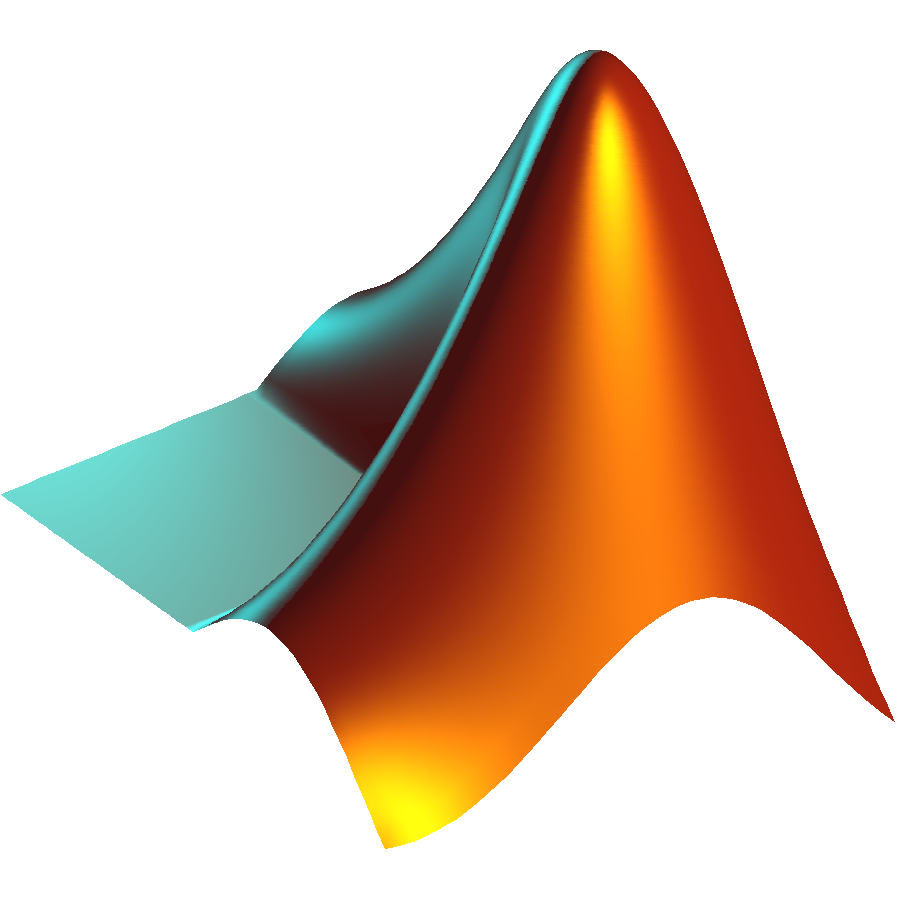
\includegraphics[width=16pt]{matlab-logo.png}};},%
     listing options={basicstyle=\footnotesize\ttfamily,breaklines=true,%
                      postbreak={\mbox{$\hookrightarrow\space$}},%
                      language=Matlab,style=MatlabStyle},%
  }%
 }%
 {\endtcblisting}

\newenvironment{python}{%
  \tcblisting{listing only,colback=c_code_colback,colframe=c_code_colframe, enlarge top by=5.5mm,enhanced,boxrule=1pt,%
     overlay={\node[anchor=west,xshift=10pt,draw=c_code_colframe, line width=2pt, rectangle, rounded corners=2pt,fill=c_code_icon_fill,inner sep=2pt,outer sep=0pt, minimum size=20pt] at (frame.north west) {
\includegraphics[width=16pt]{python-logo.pdf}};},%
     listing options={basicstyle=\footnotesize\ttfamily,breaklines=true,%
                      postbreak={\mbox{$\hookrightarrow\space$}},language=Python,style=PythonStyle},%
  }%
 }%
 {\endtcblisting}
\newenvironment{sh}{%
  \tcblisting{listing only,colback=c_code_colback,colframe=c_code_colframe, enlarge top by=5.5mm,enhanced,boxrule=1pt,%
     overlay={\node[anchor=west,xshift=10pt,draw=c_code_colframe, line width=2pt, rectangle, rounded corners=2pt,fill=c_code_icon_fill,inner sep=2pt,outer sep=0pt, minimum size=20pt] at (frame.north west) {
\includegraphics[width=16pt]{sh-logo.pdf}};},%
     listing options={basicstyle=\footnotesize\ttfamily,breaklines=true,%
                      postbreak={\mbox{$\hookrightarrow\space$}},language=sh,style=PythonStyle},%
  }%
 }%
 {\endtcblisting}


\newcommand{\triangcirc}{\tikz{
\node[circle,white,draw,inner sep=3pt] (c) {};
\node[isosceles triangle,
      white,
      fill,
      rotate=-90,
      anchor=apex,
      isosceles triangle apex angle=60,
      inner sep=1.5pt] (t) at ([yshift=0.5pt]c.south) {};}}
% 
% \makeatletter
% \renewcommand*\thelstnumber{\makebox[3em][r]{\ifnum\value{lstnumber}<10 0\fi\the\value{lstnumber}}}
% \def\three@digits#1{\ifnum#1<10 00\else\ifnum#1<100 0\fi\fi\number#1}
% \makeatother

\newenvironment{mwindow}{%
  \tcblisting{   
  enhanced,
  arc = 0pt,
  outer arc = 2pt,
  colback = white,
  colframe = matlabblue,
   listing only,
  fonttitle = \bfseries,
  listing options = {%
    language = matlab,
    style=MatlabStyle
  },
  overlay = {%
    \fill[gray!30] 
      (interior.north west)
      rectangle 
      ([xshift = 1em]interior.south west);
  },%
%   /utils/exec = {%
%     \def\thelstnumber{%
%       \texttt{\csname three@digits\endcsname{\the\value{lstnumber}}}}},
  title = {\ttfamily Command window\hfill\triangcirc}
  }%
 }%
 {\endtcblisting}

 
  % langage par défaut
\lstset{language=Matlab, style=MatlabStyle}

\def\minline{\lstinline[language=Matlab,breaklines=true]}
\def\pinline{\lstinline[language=Python,breaklines=true]}

%----------------------------------------------------------------------------------------
%	REMARK ENVIRONMENT
%----------------------------------------------------------------------------------------

% Remark with \matlabregistered{} logo
\newenvironment{mremark}{\par\vskip10pt\small % Vertical white space above the remark and smaller font size
\noindent\ignorespaces\begin{minipage}{20pt} 
   \begin{tikzpicture}[overlay]
   \node[anchor=east,draw=c_code_colframe, line width=1pt, rectangle, rounded corners=2pt,fill=c_code_icon_fill,inner sep=2pt,outer sep=0pt, minimum size=20pt] at (-10pt,0pt){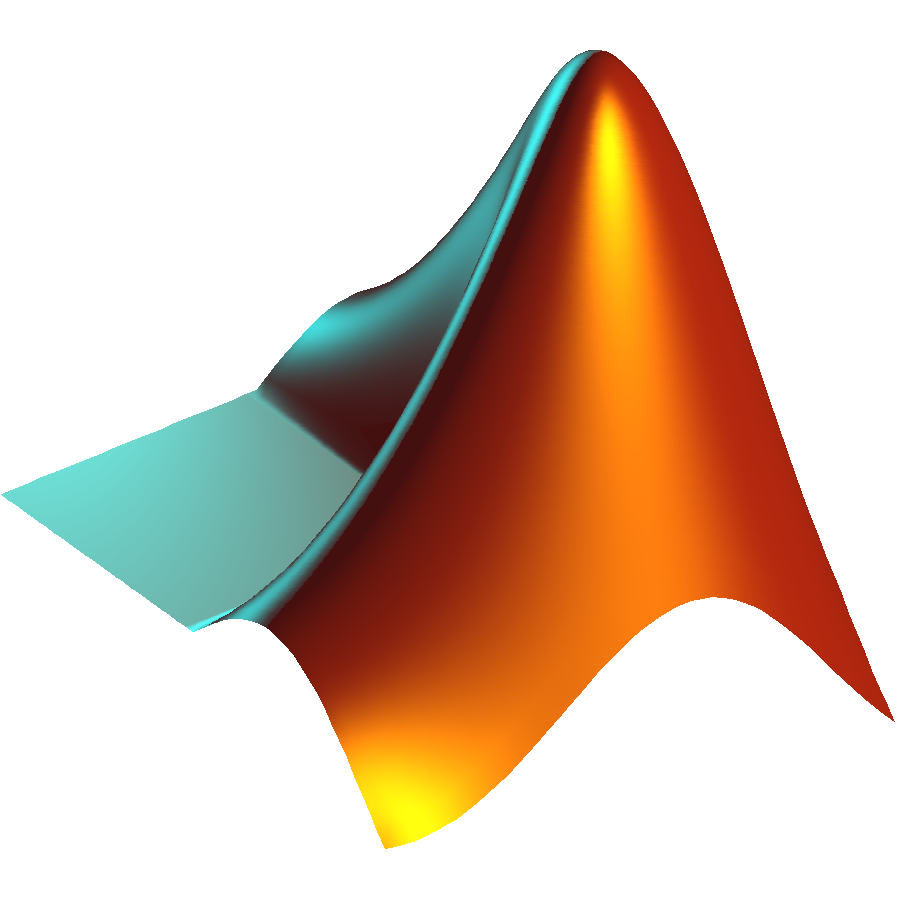
\includegraphics[width=16pt]{matlab-logo.png}};
   \end{tikzpicture}%
  \end{minipage}%
	\begin{minipage}{.8\textwidth}\flushleft
  }
{
\end{minipage}\par\noindent%
\ignorespacesafterend
\vskip12pt} % Tighter line spacing and white space after remark

% Remark with python logo
\newenvironment{premark}{\par\vskip10pt\small % Vertical white space above the remark and smaller font size
\noindent\ignorespaces\begin{minipage}{20pt}   
   \begin{tikzpicture}[overlay]
   \node[anchor=east,draw=c_code_colframe, line width=1pt, rectangle, rounded corners=2pt,fill=c_code_icon_fill,inner sep=2pt,outer sep=0pt, minimum size=20pt] at (-10pt,0pt){
\includegraphics[width=16pt]{python-logo.pdf}};
   \end{tikzpicture}%
  \end{minipage}%
	\begin{minipage}{.8\textwidth}\flushleft
  }
{
\end{minipage}\par\noindent%
\ignorespacesafterend
\vskip12pt} % Tighter line spacing and white space after remark


\newtcolorbox{qbox}[1][]{
	enhanced jigsaw,
  %width=0.5\textwidth,  %% change
  colback=c_qbox_colback,
  colframe=c_qbox_colframe,
  title={
\includegraphics[width=10pt]{interrogation.pdf}},
  boxrule=2pt,
  breakable,
  %left=10pt,right=10pt,top=20pt,bottom=20pt,
  attach boxed title to top left= {xshift=10pt,yshift*=-\tcboxedtitleheight/2},
  boxed title style={boxrule=0pt,size=small,colback=c_qbox_icon_colback,colframe=c_qbox_icon_colframe},
  before=\par\vspace{3mm},
  #1
}

\newtcolorbox{mhelp}[1][]{
	enhanced jigsaw,
  %width=0.5\textwidth,  %% change
  colback=c_code_colback,
  colframe=c_code_colframe,
  coltitle=c_code_title,
  title={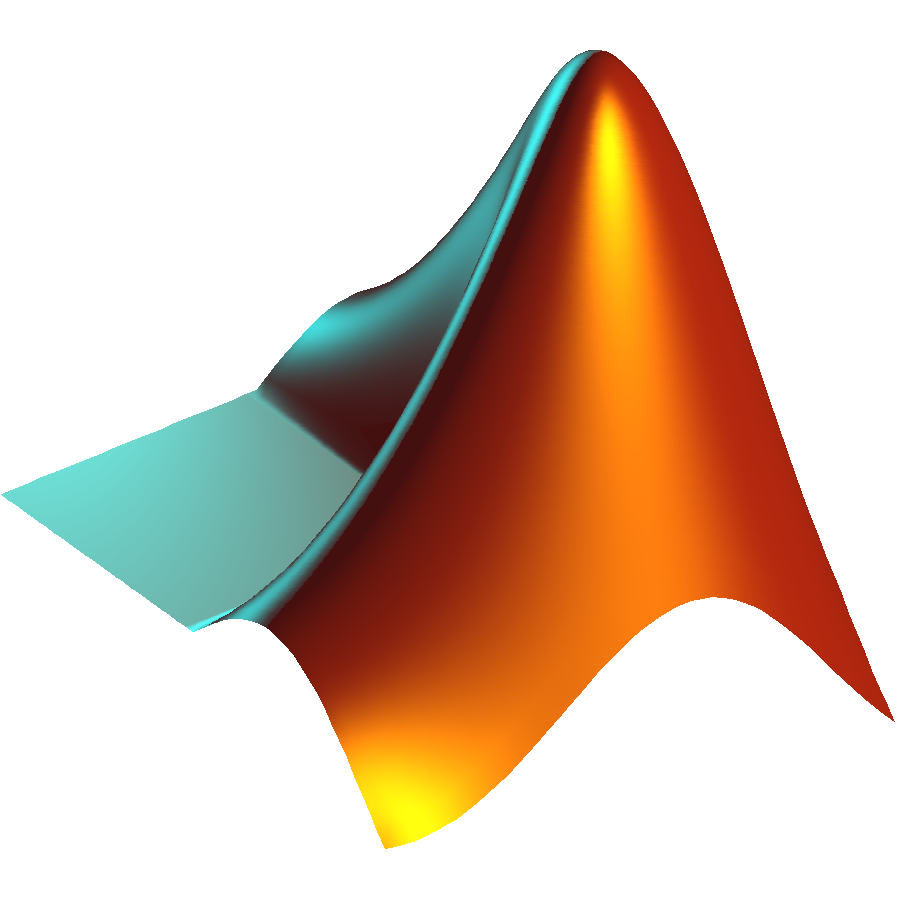
\includegraphics[width=16pt]{matlab-logo.png} Informations},
  boxrule=1pt,
  breakable,
  attach boxed title to top left= {xshift=10pt,yshift*=-\tcboxedtitleheight/2},
  boxed title style={size=small,colback=c_code_colback,colframe=c_code_colframe},
  #1
}


\newtcolorbox{phelp}[1][]{
	enhanced jigsaw,
  %width=0.5\textwidth,  %% change
  colback=c_code_colback,
  colframe=c_code_colframe,
  coltitle=c_code_title,
  title={
\includegraphics[width=16pt]{python-logo.pdf} Informations},
  boxrule=1pt,
  breakable,
  %left=10pt,right=10pt,top=20pt,bottom=20pt,
  attach boxed title to top left= {xshift=10pt,yshift*=-\tcboxedtitleheight/2},
  boxed title style={size=small,colback=c_code_colback,colframe=c_code_colframe},
  #1
}
